\ylDisplay{Mass-spektromeeter} % Ülesande nimi
{Kristian Kuppart} % Autor
{piirkonnavoor} % Voor
{2013} % Aasta
{G 10} % Ülesande nr.
{7} % Raskustase
{
% Teema: Magnetism
\ifStatement
\begin{wrapfigure}[4]{r}{3cm}%
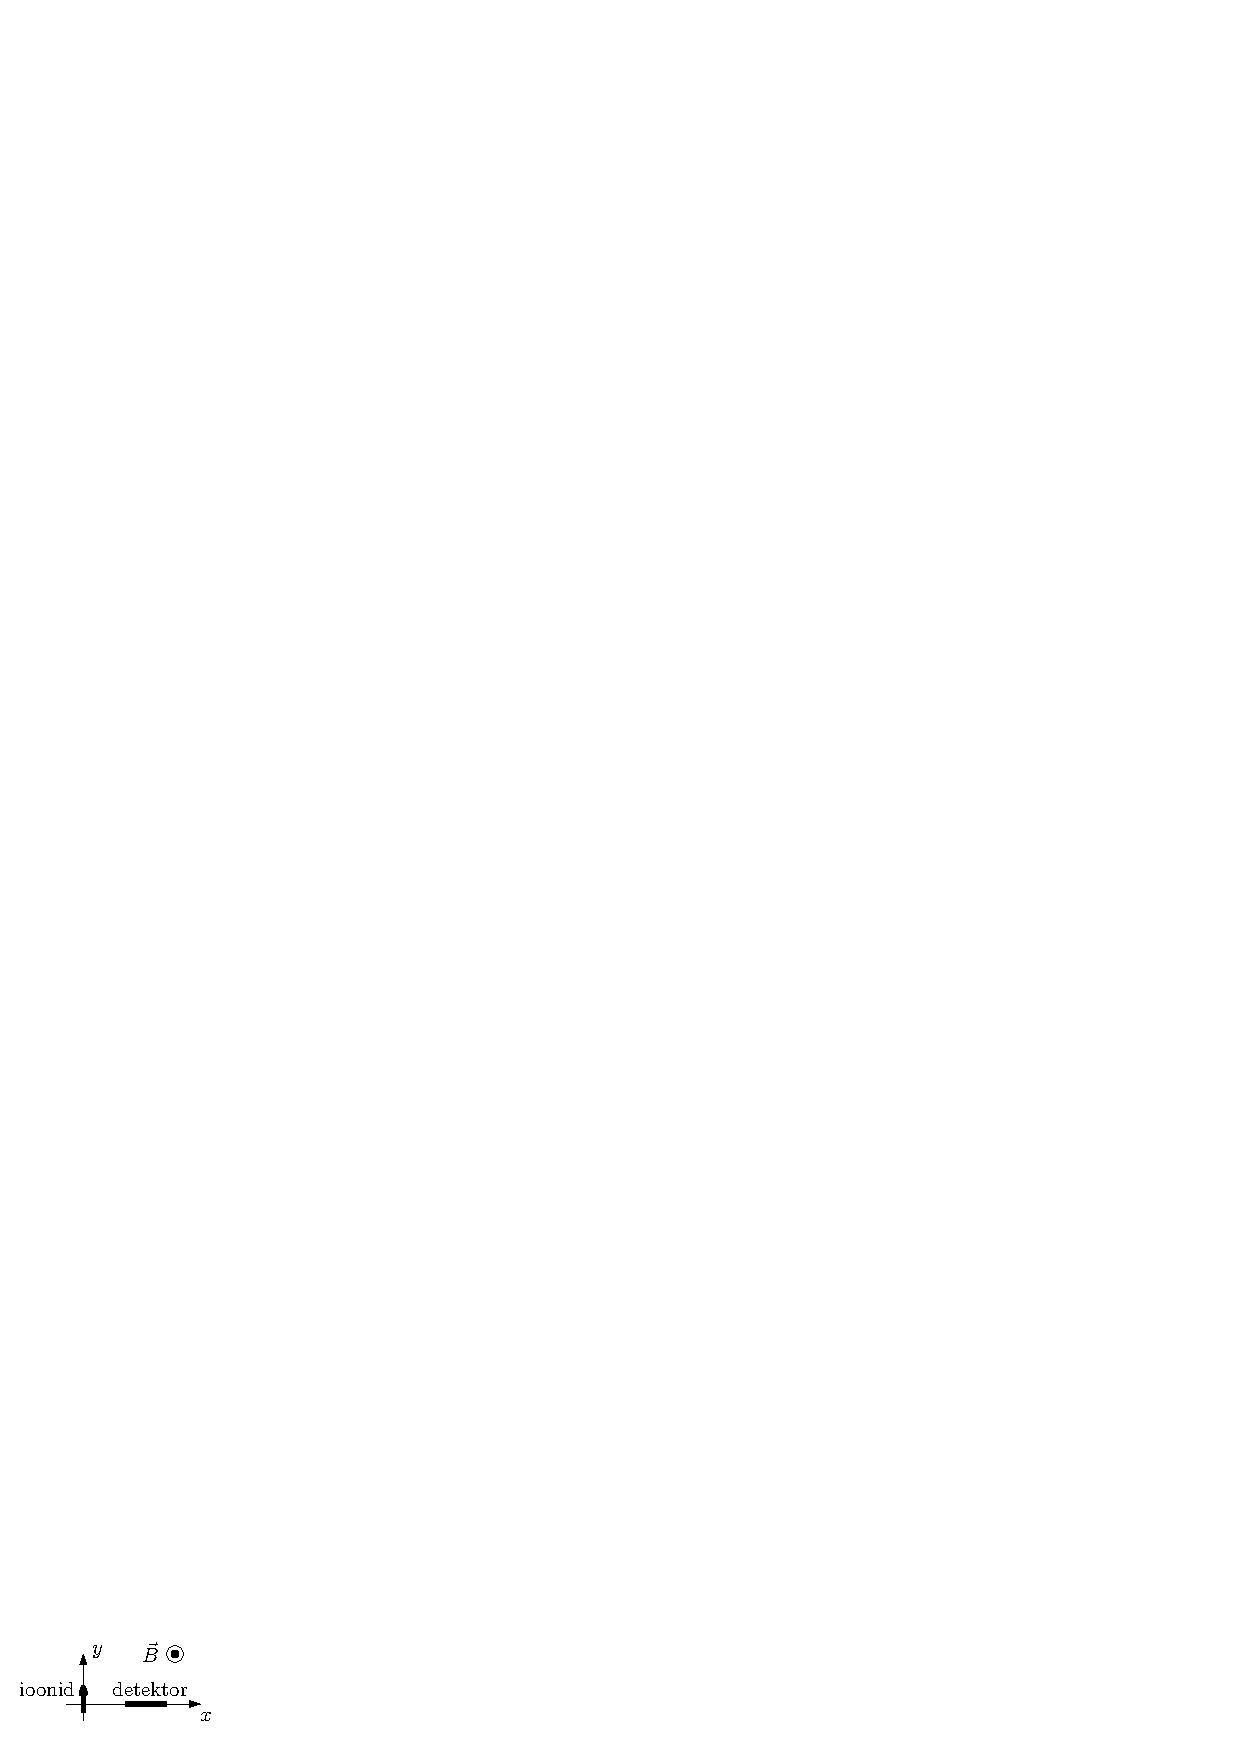
\includegraphics[width=\linewidth]{2013-v2g-10-massspektromeeter_ipe}%
\end{wrapfigure}
Laboris oli uurimiseks hulk mingit atomaarset ainet, mille molaarmassiks mõõdeti
$\mu_{1}$. Ühekordselt ioniseeritud ainet (iga aatom oli kaotanud ühe
elektroni) kiirendati elektriväljas potentsiaalide vahega $U$ ja suunati magnetvälja
induktsiooniga $B$ (vaadake joonist). Magnetinduktsioon oli joonise tasandiga
risti, 
ioonide algkiirus oli $y$-telje suunaline,
magnetväli asus piirkonnas $y>0$ ning aine sisenes magnetvälja punktis
$(0, 0, 0)$.

Täheldati, et väike kogus  ainet langes $x$-teljel asuvale
detektorile kauguse
$d$ võrra kaugemal kohast, kuhu langes põhiosa ainest. Sellest järeldati,
et aine hulgas oli väike osa isotoopi erineva molaarmassiga. Leidke
selle isotoobi molaarmass $\mu_{2}$. Avogadro arv on $N_A$ ja elektroni laeng
on $-e$.
\fi


\ifHint
Osakeste kiirus magnetvälja sisenedes on avaldatav energia jäävusest. Magnetväljas algab ringliikumine, kusjuures detektorini jõutakse pärast poole ringjoone läbimist. Teisisõnu on detekteeritud $x$-koordinaat $2R$, kus $R$ on ringjoone raadius.
\fi


\ifSolution
Potentsiaalide vahes $U$ saab kiirendatud laetud osake kineetilise
energia $\frac{mv^{2}}{2}=qU$, siit avaldame osakese kiiruse: $v=\sqrt{\frac{2qU}{m}}$. Kuna magnetväli on kiirusega risti, hakkab laetud osake 
magnetvälja jõudes liikuma seal mööda ringjoone kaart, kus ringjoone raadius
$R=\frac{mv}{qB}$. Selleks ajaks, kui osake jõuab detektorini,
on ta läbinud pool ringjoonest. Olgu $m_{2}$ raskema isotoobi
mass ja $m_{1}$ kergema isotoobi mass. Sel juhul 
\[ 
2\left(\frac{m_{1}v_{1}}{qB}-\frac{m_{2}v_{2}}{qB}\right)=d, 
\]
ehk
\[ 
m_{2}v_{2}=\frac{qBd}{2}+m_{1}v_{1 }.
\]
Arvestades, et $v_{1}=\sqrt{\frac{2eU}{m_{1}}}$ ja $v_{2}=\sqrt{\frac{2eU}{m_{2}}}$,
kus $e$ on elementaarlaeng, saame eelmise võrrandi ümber kirjutada kui
\[ \sqrt{m_{2}}=\sqrt{m_{1}}+\frac{Bd}{2}\sqrt{\frac{e}{2U}}. \]
Võttes arvesse, et $m_{2}=\frac{\mu_{2}}{N_{A}}$ ja $m_{1}=\frac{\mu_{1}}{N_{A}}$,
kus $N_{A}$ on Avogadro arv, saame:
\[ \mu_{2}=N_{A}\left(\sqrt{\frac{\mu_{1}}{N_{A}}}+\frac{Bd}{2}\sqrt{\frac{e}{2U}}\right)^{2}.\]
\fi


\ifEngStatement
% Problem name: Mass spectrometer
\begin{wrapfigure}[4]{r}{3cm}%
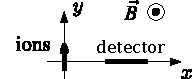
\includegraphics[width=\linewidth]{2013-v2g-10-massspektromeeter_ipe_ing}%
\end{wrapfigure}
In a laboratory there was a quantity of a substance to be examined. The molar mass of the substance was measured to be $\mu_{1}$. The substance was ionized once (each atom lost one electron), then accelerated in an electric field with a potential difference $U$ and directed to a magnetic field of induction $B$ (see figure). The magnetic induction was perpendicular to the plane of the figure, the initial velocity of the ions was $y$-directional, the magnetic field was located in the region $y>0$ and the substance entered the magnetic field at the origin, $(0, 0, 0)$.\\
It was observed that a small amount of the substance fell by a distance $d$ further on the detector on the $x$-axis from where the rest of the substance fell on. From this it was assumed that a small amount of the isotope in the substance had a different molar mass. Find the molar mass $\mu_{2}$ of this isotope. The Avogadro number is $N_A$ and the charge of an electron is $-e$.
\fi


\ifEngHint
The speed of the particles entering the magnetic field can be expressed from the conservation of energy. Circular motion begins in the magnetic field, moreover the detector is reached after covering half a circle. In other words, the detected $x$-coordinate is $2R$ where $R$ is the radius of the circle.
\fi


\ifEngSolution
In the case of potential difference $U$ an accelerated charged particle gets a kinetic energy $\frac{mv^{2}}{2}=qU$, from here we express the velocity of the particle: $v=\sqrt{\frac{2qU}{m}}$. Because the magnetic field is perpendicular to the velocity the charged particle starts to move along a circle when entering the magnetic field, the radius of the circle is $R=\frac{mv}{qB}$. By the time when the particle reaches the detector it has covered half of the circle. Let $m_{2}$ be the mass of the heavier isotope and $m_{1}$ the mass of the lighter isotope. In that case
\[ 
2\left(\frac{m_{1}v_{1}}{qB}-\frac{m_{2}v_{2}}{qB}\right)=d, 
\]
meaning 
\[ 
m_{2}v_{2}=\frac{qBd}{2}+m_{1}v_{1 }.
\]
Considering that $v_{1}=\sqrt{\frac{2eU}{m_{1}}}$ and $v_{2}=\sqrt{\frac{2eU}{m_{2}}}$ where $e$ is the elementary charge we can write the previous equation as 
\[ \sqrt{m_{2}}=\sqrt{m_{1}}+\frac{Bd}{2}\sqrt{\frac{e}{2U}}. \]
Taking into account that $m_{2}=\frac{\mu_{2}}{N_{A}}$ and $m_{1}=\frac{\mu_{1}}{N_{A}}$, where $N_{A}$ is the Avogadro constant, we get:
\[ \mu_{2}=N_{A}\left(\sqrt{\frac{\mu_{1}}{N_{A}}}+\frac{Bd}{2}\sqrt{\frac{e}{2U}}\right)^{2}.\]
\fi
}